\chapter{Résumé en Français}
\label{chap:intro-fr}

\selectlanguage{english}
\begin{kaobox}[backgroundcolor=Black!10!White,frametitlebackgroundcolor=Black!10!White]
  This \lcnamecref{chap:intro-fr} is an introduction intended for French-speaking readers.
  If your English is better than your French,
  you should instead read \cref{chap:intro-en}, its translation in English.
\end{kaobox}
\selectlanguage{french}

\emph{“\kl{Coq} est un vieil homme maintenant, et il a de nombreuses cicatrices.”}
\vspace{-1.5em}
\begin{flushright}
  \sidecite[][citant Assia Mahboubi, traduction personnelle]{QuantaPA}
\end{flushright}

\margintoc[4em]

Cette thèse se situe dans le domaine de la \kl[type dépendant]{théorie des
types}, lui-même au croisement entre informatique et logique mathématique.
Un de ses objectifs est de donner des fondements théoriques et pratiques
à des outils informatiques assistant les humains dans la construction
et la vérification de preuves – au sens mathématique du terme.
De tels outils sont appelés \kl{assistants à la preuve}, et, dans cette thèse, il sera
en particulier beaucoup question de l’un d’entre eux,
sur lequel mon travail s’est principalement concentré : \kl{Coq}.

Durant leurs plus de 50 ans d’existence, les assistants à la preuve sont devenus une
technologie établie. Avec l’évolution du domaine, les outils sont devenus de plus en
plus complexes, ce qui les rend à la fois de plus en plus puissants, mais aussi de plus
en plus sensibles à des bugs critiques cachés dans des recoins obscurs. Alors que les
assistants à la preuve sont graduellement adoptés dans un nombre grandissant de communautés
attachées à un haut niveau de fiabilité, cette situation n’est pas tenable.
La solution historique consistant à placer sa confiance dans un petit noyau fiable
– dénommé critère de De Bruijn –, n’est tout simplement pas suffisante si l’on veut avancer
en intégrant de nouvelles fonctionnalités puissantes pour suivre les besoins des utilisateurs
et utilisatrices.

Il y a une solution simple à ce problème : les assistants à la preuve sont utilisés depuis
des décennies pour certifier la correction de programmes. Pourquoi ne pourraient-ils pas
prouver \emph{leur propre} correction ? Après tout, s’il s’agit là de l’étalon ultime
pour mesurer la confiance qu’on peut accorder à un logiciel,
il devrait s’appliquer en premier lieu à ceux utilisés pour justifier cette
confiance. Pour l’assistant à la preuve \kl{Coq}, cette ambition est celle du projet
\kl{MetaCoq}, qui vise à construire un nouveau noyau pour \kl{Coq} qui soit entièrement
prouvé correct. À terme, l’objectif est tout simplement pouvoir remplacer le noyau actuel,
et on doit donc prendre en compte toute sa complexité.

Mais avant de pouvoir atteindre ce but, il est nécessaire d’étudier plus en profondeur
les structures à l’œuvre dans le noyau. En particulier, son algorithme de typage est
\emph{bidirectionnel}, ce qui signifie qu’il alterne systématiquement entre deux problèmes :
l’\emph{inférence} – trouver un type pour un terme – et la \emph{vérification} –
vérifier qu’un type donné convient pour un terme. Bien que cette structure soit cruciale pour
relier la spécification du système de type à son implémentation, elle a été relativement
peu étudiée dans le contexte du Calcul des Constructions Inductives (CIC), la fondation
théorique de \kl{Coq} – mais aussi de ses cousins \kl{Lean}, \kl{Agda}…

Cette thèse vise à remplir ce vide, en fournissant une étude rigoureuse d’un CIC
bidirectionnel, formalisée dans le cadre offert par le projet \kl{MetaCoq}. Celle-ci
est un ingrédient clé dans la première preuve de correction et de complétude d’un
algorithme de typage pour un noyau réaliste d’assistant à la preuve.
Elle a également permis de découvrir des bugs dans le noyau de \kl{Coq} qui étaient
jusque-là passés inaperçus.

Mais le typage bidirectionnel est également un outil théorique intéressant en lui-même,
donnant un contrôle précieux sur le calcul. En particulier, c’est une pièce nécessaire
dans la conception d’une extension graduelle à \kl{CIC}, \kl{GCIC}.
Le typage graduel vise à apporter aux programmeurs et programmeuses à la fois la flexibilité
de développement offerte par le typage dynamique, et les garanties fortes données par
le typage statique, dans un seul et même système. \kl{GCIC} cherche à fournir cette
flexibilité à la programmation utilisant des types dépendants, et, en utilisant la
puissance de la correspondance de Curry-Howard, à l’écriture de preuve. Mais cette
entreprise bute sur de subtiles difficultés, que seul le cadre bidirectionnel permet
de résoudre.

Pour replacer ce travail dans son contexte large, cette introduction
commence par une très courte histoire de la logique mathématique
(\cref{sec:logique-histoire}), qui expose les principales problématiques de ce domaine.
Suit une présentation des liens entre logique et informatique, par
l’intermédiaire des \kl{assistants à la preuve} (\cref{sec:assistants-preuve}).
La \cref{sec:intro-coq} s’intéresse plus particulièrement aux questions
de recherche sur lesquelles j’ai travaillé: typage bidirectionnel, \kl{MetaCoq} et typage
graduel.
Enfin la \cref{sec:cette-these} résume mes contributions à ces questions.

\section{Une très courte histoire de la logique}
\label{sec:logique-histoire}

\subsection{Les syllogismes}

La question principale à laquelle la logique cherche à répondre
est celle de trouver des critères afin de déterminer si un raisonnement est valide.
Dans la tradition occidentale, on peut faire remonter l’étude de cette problématique
à l’Antiquité, et notamment à Aristote, avec son \textit{Organon}.
L’apport majeur de ce travail est d’introduire la notion de syllogisme.
Il s’agit de fragments simples de raisonnement, dont la validité tient au fait qu’ils
suivent une structure fixée, et non à un contenu particulier.%
\sidenote{
  Le plus connu est probablement le syllogisme \textit{Barbara}, dont un exemple est :
  \emph{tous les humains sont mortels ; Socrate est humain ; donc Socrate est mortel.}
}
Si un raisonnement complexe est construit en assemblant ces syllogismes,
celui-ci pris dans son entier doit nécessairement être valide, puisque
chacun des fragments assemblés l’est. Il y a ici deux idées importantes.

La première est qu'un raisonnement peut être valide ou non du simple fait de sa structure, indépendamment de son contenu.
Il peut s’agir de syllogismes, mais aussi de bien d’autres systèmes. On en rencontrera
un certain nombre au cours cette thèse !

La seconde est celle de la construction à partir de composantes élémentaires. À
partir d’un système de règles de base qu’on a identifiées comme valides 
\textit{a priori}, on a un moyen de s’assurer de la validité
de raisonnements potentiellement très complexes.
Il suffit pour cela de vérifier que ceux-ci peuvent être décomposés en un
assemblage des composantes de base.

Pour les philosophes grecs,
la logique est également pensée comme un outil de communication.
Il s’agit de vérifier la validité de son propre raisonnement,
mais surtout de se donner le moyen d’échanger celui-ci,
en s’accordant sur un système logique formel.%
\sidenote{Les règles structurelles à respecter, comme celles des syllogismes.}
Une personne voulant que ses conclusions soient acceptées par d’autres n’a plus qu’à
exprimer son raisonnement de manière parfaitement précise dans le cadre d’un tel système.

À partir de cette époque, la logique en tant que discipline se concentre sur l’étude
de cette structure qui sous-tend le raisonnement.
L’enjeu principal est donc de construire un système formel,
adapté à un domaine de raisonnement précis. Dans le cadre qui nous intéresse,
celui de la logique mathématique, cela permet de donner un sens précis à
ce qui constitue une preuve mathématique valide.

\subsection{Les débuts de la logique mathématique : vers un fondement formel}

À la suite d’Aristote, les mathématiciens et mathématiciennes se sont donc emparés
de la logique, afin de trouver un système formel
pouvant servir de fondement rigoureux aux mathématiques.
Les liens entre logique et mathématiques remontent à l’Antiquité grecque,
mais la logique mathématique en tant que discipline indépendante s’établit réellement
durant le 19\textsuperscript{e} siècle, grâce à d’importants progrès
sur deux aspects principaux.

Le premier a consisté à se dégager du langage dit
naturel%
\sidenote{
  Par opposition aux langages formels qui apparaissent
  en mathématiques, informatique, etc.
}, inadapté à une description formellement précise de la déduction, et à
concevoir à la place une nouvelle forme de langage spécifique qui puisse servir de
base au raisonnement mathématique.
Une étape importante ici est le \citetitle{Begriffsschrift} de
\citeauthor{Begriffsschrift}~\sidecite{Begriffsschrift},
qui, le premier, donne un langage formel suffisamment riche pour exprimer les mathématiques
de manière satisfaisante. Son addition majeure est l’introduction
de la notion de quantificateur, essentielle au langage mathématique,
car ils permettent de fidèlement rendre compte des propriétés universelles%
\sidenote{Par exemple : « Tout entier pair est la somme de deux nombres premiers ».}
et existentielles%
\sidenote{Par exemple : « Il existe un réel dont le carré vaut 2 ».}.

Le second a eu pour but de montrer que les mathématiques dans leur entier peuvent
être reconstruites à partir d’un petit nombre de propriétés simples. Une étape
importante a été la réduction de l’analyse aux propriétés
des nombres réels, puis les constructions de ceux-ci à partir
de l’arithmétique données quasiment simultanément en 1872 par entre autres
Dedekind~\sidecite{Dedekind1872} et Cantor~\sidecite{Cantor1872}.
De son côté, Peano~\sidecite{Peano1889} propose
une axiomatisation des nombres entiers proche de celle encore utilisée aujourd’hui.
Enfin, Cantor à nouveau propose la théorie des ensembles~\sidecite{Cantor1883}
comme un formalisme permettant de décrire tous
les objets mathématiques sous la forme d’ensemble d’éléments.

\subsection{La crise des fondements}
Hélas, le système proposé dans le \citetitle{Begriffsschrift} est incohérent%
\sidenote{
  C’est-à-dire qu’il permet de prouver le faux, et, en conséquent, toutes les propositions,
  faisant s’écrouler le système logique – ce qui est connu sous le nom de principe d’explosion.
  Il ne peut donc servir de fondement satisfaisant aux mathématiques.
} !
Ce constat, fait par Russell en 1903%
\sidenote{
  Dans une lettre à Frege dont ce dernier rend les résultats
  publics~\cite[Nachwort p.~253]{Frege1903}.}%
\margincite{Frege1903}
ouvre une période de crise, en remettant en doute les systèmes qui avaient commencé à
s’imposer comme de bons candidats pour servir de fondements aux mathématiques –
celui de Frege, mais surtout ceux de Cantor, affectés par les mêmes difficultés.

Une possible solution est avancée dix ans plus tard
par Russell et Whitehead dans leur \citetitle{Whitehead1913}~\sidecite{Whitehead1913},
un énorme travail qui, non seulement, propose un système
formel qui évite l’incohérence du
\citetitle{Begriffsschrift}, mais qui, de plus, construit
dans ce système une quantité importante de mathématiques,
en particulier, une construction des entiers, de l’arithmétique et
finalement des nombres réels.

En parallèle, dans la continuité des travaux de Cantor,
Zermelo~\sidecite{Zermelo1908} et
d’autres travaillent à fournir une version de la théorie des ensembles de Cantor
qui soit cohérente. Ceci aboutit à ce qu’on appelle actuellement la
théorie des ensembles de Zermelo-Fraenkel – ZF, ou ZFC quand on y ajoute l’axiome
du choix \sidecite{Zermelo1904}%
\sidenote{Un axiome très utile dans de nombreuses branches des mathématiques, mais qui
est souvent traité séparément, car il est à la fois moins crucial que les autres axiomes de
ZF et à l’origine de résultats contre-intuitifs.}
–, qui semble également à même de fournir une base solide pour fonder les
mathématiques.

\subsection{L’incomplétude}

La recherche d’un système formel adéquat pour servir de fondement aux mathématiques 
se heurte cependant à une seconde difficulté majeure : le théorème d’incomplétude de
Gödel~\sidecite{Goedel1931}. Celui-ci affirme que tout système formel
dans lequel on peut construire des nombres entiers comme ceux de Peano – donc
\textit{a fortiori} tout système suffisamment riche pour fonder les mathématiques –
ne peut pas démontrer sa propre cohérence%
\sidenote{À moins qu’il ne soit incohérent, auquel cas il peut \emph{tout} démontrer.}.
De ce fait, il n’existe pas de
système qui puisse servir de base aux mathématiques
avec une certitude formelle sur son adéquation.
En effet, puisqu’on ne peut pas prouver la cohérence du
système dans lui-même, il pourrait finalement s’avérer incohérent, ruinant les
efforts fournis – exactement ce qui est arrivé au \citetitle{Begriffsschrift} de Frege.

Une conséquence de ce théorème est qu’un système suffisamment riche
pour fonder les mathématiques est nécessairement incomplet.%
\sidenote{
  Cela signifie qu’il
  existe des énoncés indépendants, à savoir des assertions qui ne sont ni démontrables,
  ni réfutable – c’est-à-dire dont la négation est démontrable.
  La cohérence du système considéré en est un exemple.
}
Ainsi, dans la suite, il ne sera jamais question de vérité dans un sens absolu –
ce qui n’aurait de sens que dans un système complet
où tout énoncé est vrai ou faux –, mais
uniquement de prouvabilité \emph{relativement à un système donné}.

\subsection{Une situation satisfaisante ?}

Malgré les difficultés mises à jour au début du 20\textsuperscript{e}
siècle, les recherches en logique mathématique ont abouti à une situation
globalement assez satisfaisante. D’abord, ZFC fournit un système formel raisonnable sur
lequel fonder les mathématiques. Ensuite,
la communauté mathématique est globalement convaincue qu’il serait
\emph{théoriquement} possible de rédiger les mathématiques dans leur ensemble
en utilisant celui-ci. Cela suffit amplement à la plupart de ses membres,
même si rares sont ceux se risquent à véritablement tenter l’expérience, dans la veine
des \citetitle{Whitehead1913}.

En \emph{pratique}, les choses sont toutes autres.
Le développement et la vérification humaine de mathématiques
formalisées%
\sidenote{C’est-à-dire effectivement exprimées dans un système formel fixé.}
semble à la fois impossible et inutile.
D’un côté, cela demanderait un effort considérable, car de telles mathématiques
nécessiteraient un niveau de précision extrêmement élevée, tant de la part de l’autrice
de la preuve formelle que de sa lectrice.
Dans le même temps, cela ne permettrait pas de réduire de manière significative
les risques d’erreurs. Il serait en effet
humainement très difficile de vérifier qu’un raisonnement suit bien les règles du
système : une minuscule erreur peut facilement se cacher au milieu de
milliers de pages de raisonnement formel.
Enfin, décrire les mathématiques de cette façon noierait
les intuitions mathématiques importantes, rendant la communication stérile.

Si on veut rendre les mathématiques formelles praticables, il faut donc développer
de nouveaux outils.

\section{Les ordinateurs entrent en scène}
\label{sec:assistants-preuve}

Un nouvel élément vient cependant modifier radicalement cette situation :
l’avènement des ordinateurs. En effet, l’informatique donne accès à de nouveaux outils,
qui permettent de rendre à la fois possible et attrayante la formalisation
des mathématiques.

\subsection{Les assistants à la preuve}

Les ordinateurs excellent là où les humains pèchent : leur spécialité est de traiter
d’immenses volumes d’information de façon très précise, exactement le type
de besoins que soulève la manipulation de mathématiques formalisées. C’est pourquoi dès
le début des années 70%
\sidenote{Avec des systèmes comme Automath~\cite{DeBruijn1970}
ou Mizar~\cite{Rudnicki1992}.}%
\margincite{DeBruijn1970}%
\margincite{Rudnicki1992}
ont commencé à apparaître des outils informatiques servant à écrire et vérifier ces
preuves formelles, que l’on appelle collectivement des \intro{assistants à la preuve}.
Via la formalisation des preuves et la vérification par l’ordinateur qu’elles
suivent bien les règles du système logique sous-jacent, les assistants à la preuve
donnent accès à une fiabilité bien plus élevée que celle permise par les preuves
“informelles”.
Des mathématiciens reconnus, comme \sidetextcite{Voevodsky2010},
\sidetextcite[][Preface, p. xi]{Hales2012}, ou \sidetextcite{Scholze2021}
se sont d’ailleurs déjà emparés des assistants à la preuve,
notamment dans le but de lever les incertitudes
quant à la solidité de leur propre travail.

De plus, le terme d’\emph{assistant} à la preuve n’a pas été choisi au hasard : au-delà
de la simple vérification, ils mettent à la disposition des
utilisateurs et utilisatrices un large éventail d’outils pour
faciliter la conception de preuves formelles.
Ces outils permettent d’écrire
les preuves à haut niveau et de manière interactive,%
\sidenote{Dans la plupart des assistants à la preuve modernes, la preuve finale est
  construite comme le résultat d’un échange entre la programmeuse et l’outil,
  plutôt qu’écrite d’un seul bloc.}
en laissant à l’assistant à la preuve le soin de construire les preuves formelles.
Il peut s’agir de simples facilités
comme la possibilité de pouvoir visualiser la structure des
preuves, de suivre l’utilisation des hypothèses, ou de techniques beaucoup plus ambitieuses.

En effet l’informatique rend possible
l’automatisation de pans entiers de l’écriture de preuves,
par exemple via l’utilisation d’un langage de tactiques \sidecite{Delahaye2000},
qui permet de programmer la génération de preuves.
La construction automatique de preuve est par ailleurs un domaine de recherche à part entière,
et la question de son intégration dans les assistants à la
preuve y est un sujet actif \sidecite{Blanchette2016,Ekici2017}.
L’informatique a également fait ses preuves dans le champ du calcul mathématique
(calcul formel, analyse numérique), et là encore des connexions prometteuses
avec les assistants à la preuve commencent à voir le jour \sidecite{Lewis2022,Mahboubi2019}.

Enfin, si l’utilisation de l’informatique facilite l’écriture de preuve,
les assistants à la preuve ouvrent inversement
de nouvelles possibilités pour la programmation.
Ils offrent en effet un cadre naturel dans lequel décrire au même endroit
le code source d’un programme, sa spécification et la preuve formelle que cette 
dernière est remplie. On peut alors \emph{prouver} que le
programme s’exécute correctement, sans rencontrer de bug.
Cette certitude mathématique est bien plus fiable que n’importe quelle batterie de tests !
Dans ce domaine, de nombreux projets ont déjà abouti à des programmes d’envergure,
entièrement prouvés corrects : compilateur pour le langage C \sidecite{Kaestner2017},
protocoles cryptographiques \sidecite{Bhargavan2017},
résolution d’équations différentielles \sidecite{Immler2018}…

\subsection{Logique, programmation et théorie des types}

Pour fonctionner, les assistants à la preuve nécessitent comme fondement un système
formel, correspondant aux “règles du jeu” mathématique qu’ils sont censés imposer.
Ainsi, ils requièrent une étude renouvelée de la logique mathématique, mais dans le but
pratique de construire des outils à la fois fonctionnels,
puissants et faciles à utiliser.
Il existe plusieurs familles d’assistants à la preuve, basées sur des
systèmes formels relativement différents. Celle qui m’intéresse dans cette thèse
est fondée sur la \kl{correspondance de Curry-Howard}
et la \kl[type dépendant]{théorie des types dépendants}.
C’est à elle qu’appartient l’assistant à la preuve \kl{Coq}
\sidetextcite{CoqDevelopmentTeam2022} qui est au cœur de mon travail.

Si on compare un programme informatique à un texte dans une langue naturelle,
les \intro(fr){types} sont une sorte d’équivalent des catégories grammaticales.
Cependant, contrairement aux langues naturelles, ces types sont conçus
en même temps que le langage de programmation,
de manière à refléter des propriétés des objets manipulés par celui-ci.
Cela permet en premier lieu de détecter des erreurs manifestes.
Par exemple, si une procédure attendant un objet de type “image” est
appliquée à un objet de type “chaîne de caractères”, une erreur pourra être rapportée
à la programmeuse.\sidenote{
  Un slogan dû à \textcite{Milner1978} affirme que
  « Les programmes bien typés ne peuvent pas  mal s’exécuter. »
}%
\margincite{Milner1978}
Mais les types sont très versatiles, et leur capacité à encoder
des propriétés des programmes sous-jacents peut servir à la compilation, la
documentation, et bien d’autres choses.
Dans notre cadre, par exemple, les types correspondent à la validité d’un raisonnement logique.

\begin{marginfigure}

  % \begin{mathpar}
  %   \inferrule{ \Gamma, A \vdash B}{\Gamma \vdash A \Rightarrow B} \and
  %   \inferrule{\Gamma \vdash A \Rightarrow B \\ \Gamma \vdash A}{\Gamma \vdash B} \and
  %   \inferrule{\Gamma, x : A \vdash t : B}{\Gamma \vdash \lambda x : A . t : A \to B} \and
  %   \inferrule{\Gamma \vdash f : A \to B \\ \Gamma \vdash u : A}{\Gamma \vdash f~u : B}

  % \end{mathpar}

  % \caption{Règles d’inférence pour l’implication et de typage des fonctions}

  \begin{mathpar}
    \inferrule{A \\ B}{A \wedge B} \and
    \inferrule{A \wedge B}{A} \and
    \inferrule{A \wedge B}{B} \\
    \inferrule{a \ty A \\ b \ty B}{(a,b) \ty A \times B} \\
    \inferrule{p \ty A \times B}{p.1 \ty A} \and
    \inferrule{p \ty A \times B}{p.2 \ty B}
  \end{mathpar}
  
  \caption{Règles d’inférence pour la conjonction et de typage pour les paires}
  \label{fig:curry-howard-exemple}
\end{marginfigure}

Cette idée est celle de la \intro{correspondance de Curry-Howard}.%
\sidenote{Explicitée la première fois dans des notes informelles de Howard datant de 1969,
publiées bien plus tard \cite{Howard1980},
reprenant des remarques antérieures de Curry \cite{Curry1958}.}%
\margincite{Howard1980}%
\margincite{Curry1958}
Plutôt qu’un théorème précis, il s’agit d’un concept très général,
selon lequel il existe une ressemblance forte entre d’un côté le monde de la
logique et des preuves, et de l’autre celui des programmes et de leurs types.
On parle aussi d’ailleurs également de \reintro{correspondance preuves-programmes}.

Un exemple valant mieux qu’un discours abstrait, on peut voir la correspondance à l’œuvre dans la \cref{fig:curry-howard-exemple}, sous la forme de règles d’inférence
ou de typage : chaque bloc présente une règle, avec au-dessus de la barre les
hypothèses, et en dessous la conclusion.
Les trois premières règles gouvernent la conjonction logique “et”, notée $\wedge$.
La première signifie que pour déduire la proposition $A \wedge B$ (“$A$ et $B$”),
il suffit de déduire $A$ et $B$ individuellement.
À l’inverse si on a comme hypothèse $A \wedge B$, alors on peut déduire à la fois $A$, et $B$.
Les trois dernières règles gouvernent le type des paires $A \times B$.
Une paire $(a,b)$ construite à partir d’un premier objet $a$ de type $A$%
\sidenote{Ce qui est noté $a \ty A$.}
 et d’un second objet $b$ de type $B$ a le type $A \times B$.
À l’inverse si $p$ est de type $A \times B$, alors on peut en récupérer la première composante
$p.1$, qui est de type $A$ et sa seconde $p.2$, de type $B$.
Si on efface les termes\sidenote{
  Dans ce contexte, on parle souvent de \emph{termes} plutôt que de programmes,
  mais les deux sont synonymes.
} des règles du bas, on obtient \emph{exactement} les règles du haut !
Ainsi, la concept de paire en programmation correspond directement à celui de conjonction
en logique : la preuve d’une conjonction est une paire de preuves.

Ceci s’étend bien au-delà du cas de la conjonction,
à une correspondance générale entre d’une part les énoncés de la logique et leurs preuves,
et d’autre part les types et les programmes. On peut voir les énoncés comme des types,
et une preuve d’un énoncé comme un programme ayant le type qui lui correspond – ou l’inverse !
Au-delà de la simple analogie entre formalismes d’origines différentes, cette correspondance est un outil puissant pour faire dialoguer deux mondes.
En particulier, elle permet de relier deux problèmes \textit{a priori} éloignés :
vérifier qu’une preuve est correcte, et vérifier qu’un terme est bien typé.
Dans les deux cas, il s’agit de vérifier qu’une construction – programme d’un côté,
preuve de l’autre – respecte un ensemble de règles formelles garantissant qu’elle est
bien formée.

La \kl{correspondance de Curry-Howard} est donc idéale pour servir de fondements aux
assistants à la preuve, puisqu’elle permet de voir un système formel
comme une logique, tout en donnant accès à des idées venant de
la large littérature sur les langages de programmation, notamment
la théorie et l’implémentation des systèmes de types.
Dans ce cadre, les \intro[type dépendant]{systèmes de types dépendants} 
forment une famille particulière de systèmes de types, dont la
caractéristique principale est d’autoriser les types à dépendre de termes.
L’exemple archétypique du point de vue de la  programmation est le type
$\Vect(A,n)$ des vecteurs de longueurs $n$,
les listes contenant exactement $n$ éléments de type $A$ – avec $n$ un entier.
Ce type dépend de $n$, au sens où ses habitants diffèrent suivant ses valeurs.
Du point de vue de la logique, cette
dépendance correspond à la quantification : si on veut exprimer
une propriété universelle « pour tout $x$, on a $P(x)$ », on a besoin que la propriété $P$
puisse dépendre de $x$.
Grâce à cette capacité à exprimer la quantification,
les types dépendants sont suffisamment riches et puissants pour
servir de fondement aux mathématiques.

\section{\kl{Coq} et son noyau}
\label{sec:intro-coq}

Intéressons-nous maintenant un peu plus précisément à l’assistant à la
preuve dont il sera le plus question dans cette thèse : \kl{Coq}.

\subsection[Le noyau]{Le noyau, clé de voûte du système}

\begin{figure}[h]
  \centering
  \includegraphics{./figures/coq-kernel-fr.pdf}

  \caption{L’architecture schématique de \kl{Coq}}
  \label{fig:coq}
\end{figure}


\kl{Coq} est basé sur la \kl{correspondance de Curry-Howard} : les preuves sont vues comme des programmes dans un langage appelé \intro(fr){Gallina},
et leur vérification est effectuée par un algorithme proche
de ceux utilisés pour les types des langages conventionnels.
Cependant, si, dans les premières versions des années 80, \kl{Coq} ressemblait à un langage de programmation un peu étrange, ce n’est actuellement plus du tout le cas.
La raison est que la majeure partie de l’outil dans ses versions actuelles a
pour but d’aider l’utilisatrice à générer une preuve correcte. C’est un véritable
\kl[assistant à la preuve]{\emph{assistant} à la preuve} !
% \begin{marginfigure}
%   \begin{center}
%     \includegraphics[width=\textwidth]{coq-kernel-fr.pdf}
%   \end{center}
% \end{marginfigure}
Ce fonctionnement est illustré ci-contre : l’utilisatrice échange interactivement avec \kl{Coq}, qui utilise cette interaction pour générer un terme de preuve. Celui-ci est ensuite envoyé à une partie bien spécifique de l’outil, appelée \intro{noyau}.
C’est lui qui implémente l’algorithme de vérification de type, et s’assure ainsi de la correction des termes de preuve construits interactivement.
Le \kl{noyau} est donc l’élément crucial de \kl{Coq}, car c’est lui – et lui seul – qui est responsable en dernier lieu de la validation des preuves.

Cette architecture, qui isole clairement la partie critique du système,
est appelée \intro{critère de De Bruijn}~\sidecite{Barendregt2001} en 
hommage à l’un des pionniers des assistants à la preuve.
% Elle a permis de mener à bien des projets de grande ampleur, parmi lesquels CompCert~\sidecite{Kaestner2017} – un compilateur optimisant pour le langage C entièrement prouvé correct –, ou les preuves du théorème des quatre couleurs~\sidecite{Gonthier2007} et du théorème de l’ordre impair~\sidecite{Gonthier2013}, deux théorèmes importants et difficiles respectivement de la théorie des graphes et des groupes.
Si le reste de l’écosystème s’est beaucoup plus développé que le \kl{noyau} depuis les débuts, celui-ci a également évolué, en se complexifiant graduellement.
Et comme tout développement logiciel, il n’est pas à l’abri de bugs\sidenote{De l’ordre d’un bug détecté par an, une liste est maintenue à l’adresse suivante : \url{https://github.com/coq/coq/blob/master/dev/doc/critical-bugs}.}.
Ceux-ci sont en général difficilement exploitables par une utilisatrice,
encore plus sans s’en rendre compte.
Néanmoins, ils existent,
et le \kl{noyau} tendant à toujours plus se complexifier
ils risquent de continuer à apparaître.

\subsection{\kl{MetaCoq}, une formalisation en \kl{Coq}, pour \kl{Coq}}[\kl{MetaCoq}]
\label{sec:intro-metacoq}


Si on veut garantir un niveau de fiabilité le plus élevé possible, il faut donc de nouvelles idées.
Le projet \intro{MetaCoq}, a pour but de répondre à cette problématique.
L’approche est simple : il s’agit d’utiliser \kl{Coq} lui-même pour certifier la correction de son \kl{noyau}.

Plus précisément, la première étape est de décrire le système de type sur lequel est basé le \kl{noyau}, puis de démontrer ses propriétés théoriques.
% , comme la confluence de la réduction, la préservation du typage par cette même réduction, etc.
Une fois ces propriétés établies, la deuxième étape
% \sidenote{C’est celle sur laquelle j’ai principalement travaillé, et sur laquelle 
% on reviendra plus longuement.}
consiste à implémenter un algorithme de vérification de type ressemblant au maximum à celui du \kl{noyau}, directement en \kl(fr){Gallina}\sidenote{
  En effet, grâce à la \kl{correspondance de Curry-Howard}, \kl(fr){Gallina} est certes un langage
  de preuve, mais aussi un véritable langage de programmation !}.
On démontre en même temps qu’il est bien \reintro(bidir){correct}%
\sidenote{
  Si l’algorithme prétend qu’un terme est bien typé, alors c’est bien le cas.}
et \reintro[Completeness]{complet}%
\sidenote{L’algorithme répond bien affirmativement sur tous les termes bien typés.}.
Enfin, lors d’une troisième étape, on extrait de ce programme \kl(fr){Gallina} certifié
un autre programme plus efficace, en effaçant le contenu lié à la preuve de correction
pour ne garder que celui qui est algorithmiquement intéressant.
Cette extraction est une étape complexe,
mais cruciale si on veut remplacer le \kl{noyau} actuel en conservant une
efficacité raisonnable.
C’est pourquoi on prouve là encore que ladite extraction est correcte%
\sidenote{C’est-à-dire qu’elle préserve la sémantique des programmes.},
en la programmant à nouveau en \kl(fr){Gallina}.

\subsection{Vérification, inférence et typage bidirectionnel}[Typage bidirectionnel]

Durant la deuxième étape, afin de prouver que l’algorithme de typage est complet,
il est très utile de
passer par une spécification intermédiaire plus structurée que la description
théorique de la première étape.
En particulier, il est important de séparer deux questions proches, mais
bien distinctes :
d’une part, la vérification, où on cherche à \emph{vérifier}
qu’un terme a bien un type donné ;
d’autre part, l’inférence, où on cherche à \emph{trouver}
un type pour un terme, s’il existe.
L’algorithme de typage du \kl{noyau} de \kl{Coq} est \intro{bidirectionnel},
c’est-à-dire qu’il alterne en permanence entre ces deux questions
lorsqu’il vérifie qu’un terme est bien typé.
% Par exemple, dans le cas d’une application $f~u$, il commence par inférer un type pour $f$, vérifie qu’il s’agit d’un type produit $\P x : A . B$ (une généralisation du type fonctionnel $A \to B$), puis vérifie que $u$ a le type $A$.
Cette structure bidirectionnelle étant plus proche de l’algorithme,
la décrire formellement mais séparément de l’implémentation
permet de bien diviser les difficultés entre, d’un côté, son équivalence avec la présentation
d’origine, et, de l’autre, la partie purement liée aux questions d’implémentation.

Dans le cas spécifique des types dépendants, bien que présent depuis l’origine dans les algorithmes de vérification de type~\sidecite{Huet1989},
le typage bidirectionnel a été relativement peu étudié.
Pourtant, au-delà de son lien fort avec les algorithmes,
cette approche présente également des avantages théoriques : elle permet,
par sa structure plus contrainte que la présentation standard,
d’obtenir des propriétés difficiles à démontrer dans ce cadre.

\subsection{Types graduels : un peu de flexibilité dans un monde désespérément statique}
  [Types graduels]
\label{sec:intro-graduel}

Il existe deux grandes approches de la vérification du type des programmes.
Dans l’approche statique\sidenote{Qui est celle sur laquelle est basée \kl{Coq}.},
les types sont vérifiés en amont de l’exécution, alors que, dans l’approche dynamique, le bon typage des opérations est vérifié à la volée lors de cette même exécution.
La discipline dynamique est plus flexible, parce qu’elle permet de vérifier exactement ce qui est nécessaire à la bonne exécution d’un programme.
La rigidité du typage statique permet, elle, de détecter des erreurs plus tôt dans le développement, et impose des invariants utiles pour optimiser la compilation ou l’exécution.
Plutôt que d’opter exclusivement pour l’une de ces deux approches,
le \intro{typage graduel}~\sidecite{Siek2015} vise à intégrer
dans un même langage disciplines statiques et dynamiques.
L’idée est d’avoir une première passe de vérification avant l’exécution, comme en typage statique, tout en laissant la possibilité de déférer une partie de la vérification à l’exécution, comme en typage dynamique.
On a alors accès à tout un spectre d’options,
d’une discipline totalement statique à une discipline totalement dynamique,
en pouvant choisir finement quelles parties d’un programme on veut vérifier de quelle façon.
En particulier, on peut faire évoluer la discipline au fur et à mesure d’un développement
logiciel, pour bénéficier de la flexibilité du typage dynamique dans les phases précoces et des
garanties du typage statique par la suite.

Comme le cas de \kl{MetaCoq} l’illustre, \kl{Coq} peut être utilisé comme un véritable langage
de programmation. Mieux : son système de type 
permet d’exprimer des propriétés très complexes des programmes, et ainsi de vérifier
avant même leur exécution que celles-ci sont bien respectées par le code.
Hélas, cette impossibilité d’écrire du code imparfait peut
se retourner contre l’utilisatrice, en rendant plus difficile la phase de développement.
En effet, personne n’écrit du code totalement correct au premier essai,
et il serait parfois bon de pouvoir lever temporairement
les garanties très fortes du typage afin de faciliter l’expérimentation.
L’idée serait alors de s’inspirer des idées du typage graduel, pour permettre un développement
logiciel ou logique plus flexible. Ici encore, la \kl{correspondance de Curry-Howard}
est à l’œuvre, puisqu’on adapte des concepts venant du monde de la programmation
au cadre de la logique.

\section{Et cette thèse, alors ?}
\label{sec:cette-these}

Mon travail de doctorat lui-même
est centré principalement autour du typage bidirectionnel, sous
trois aspects, correspondant aux trois parties de cette thèse.
Elles sont précédées par le \cref{chap:intro-en}, version anglophone
de ce chapitre, et le \cref{chap:tech-intro}, qui introduit les principales
notions techniques utilisées dans la suite.

\subsection{Théorie du typage bidirectionnel}

La première partie (\nameref{part:bidir}) propose de combler une partie du
manque de travail théorique autour du typage bidirectionnel pour les types dépendants.
Elle contient en particulier une
preuve d’équivalence entre la présentation standard de la littérature
et une présentation bidirectionnelle.
Le \cref{chap:bidir-ccw} présente les idées générales qui guident ce travail
dans un cadre relativement simple, afin de faciliter leur exposition. 
Le \cref{chap:bidir-pcuic} montre comment étendre ces idées à un
cadre plus réaliste, proche de la théorie des types implémentée en pratique dans \kl{Coq}.
Enfin le \cref{chap:bidir-conv} traite du statut particulier de la
conversion\sidenote{Cette notion cruciale permet d’intégrer dans la
  théorie des types dépendants l’idée de calcul des programmes.}
et des liens entre certains travaux récents sur ce sujet et le typage bidirectionnel.

\subsection{Typage bidirectionnel dans \kl{MetaCoq}}

La seconde partie de cette thèse (\nameref{part:metacoq})
concerne le projet \kl{MetaCoq},
et en particulier la formalisation en \kl{Coq} des idées présentées dans la
première partie. Le \cref{chap:metacoq-general} donne une présentation générale du
projet, tandis que le \cref{chap:kernel-correctness} se concentre spécifiquement
sur la preuve que le \kl{noyau} implémenté par \kl{MetaCoq} respecte sa spécification.

\subsection{Élaboration bidirectionnelle pour le typage graduel}

Enfin la troisième et dernière partie (\nameref{part:gradual})
présente mon travail dans le domaine des \kl{types graduels}.
Les types dépendants formant déjà des systèmes
complexes, l’adaptation de ceux-ci à l’approche graduelle est particulièrement
délicate. Un résumé des possibilités et problématiques associées est présenté
en \cref{chap:gradual-dependent}.
Un point intéressant à souligner est que la présentation habituelle
des types dépendants s’avère inadaptée, car trop flexible.
La structure additionnelle apportée par le typage bidirectionnel est donc importante.
Elle est de plus apparue comme pertinente pour présenter
l’élaboration de termes depuis un langage source dans un langage cible, une
caractéristique importante des \kl[graduel]{langages graduels}.
L’utilisation d’une élaboration bidirectionnelle, et les propriétés qu’elle
permet d’obtenir, sont décrites en \cref{chap:bidir-gradual-elab}.
Enfin le \cref{chap:beyond-gcic} décrit succinctement le reste des travaux auxquels
j’ai participé dans le cadre des types graduel, mais qui n’est pas directement lié
au typage bidirectionnel.

\subsection{Contributions techniques}

Mon travail de doctorat a débuté avec l’étude des types \kl(typ){dépendants} \kl{graduels}.
J’ai contribué avec Kenji Maillard, Nicolas Tabareau et Éric Tanter à
\sidetextcite{LennonBertrand2022}, où nous étudions une extension graduelle
pour le Calcul des Constructions Inductives. Ma contribution technique principale
dans ce cadre correspond au \cref{chap:bidir-gradual-elab}.
Le \cref{chap:gradual-dependent} est également tiré de cette publication.
Un second article, avec les mêmes auteurs et dans la continuité du précédent,
est actuellement en phase de relecture. Il en sera rapidement question au
\cref{chap:beyond-gcic}, ainsi que de la seconde partie technique de
\textcite{LennonBertrand2022}, dont le contributeur principal est Kenji Maillard.

Ce travail ayant montré l’utilité d’un système de type bidirectionnel dépendant
et le manque de résultats sur le sujet, j’ai choisi de l’étudier
plus en détail, à la fois sur papier et par le biais d’une
formalisation se basant sur \kl{MetaCoq}.
Ceci a donné lieu à une seconde publication~\sidecite{LennonBertrand2021},
et correspond aux \cref{chap:bidir-ccw,chap:bidir-pcuic}, ainsi qu’à une partie du
\cref{chap:kernel-correctness}.

J’ai ensuite travaillé à l’intégration de cette formalisation à
\kl{MetaCoq}, et à son utilisation dans l’optique de montrer la complétude du \kl{noyau}
qui y est implémenté. Ceci correspond au reste du \cref{chap:kernel-correctness}.
Au-delà de cette contribution principale,
j’ai également participé à ce projet sur d’autres points plus mineurs.
Cette partie de mon travail de thèse n’a pas encore été publiée, mais
les autres contributeurs de \kl{MetaCoq} et moi-même y œuvrons actuellement.

Enfin le \cref{chap:bidir-conv} correspond à un projet que j’ai entamé dans
le but d’étendre \kl{MetaCoq}, mais qui n’a pas encore atteint le stade de la
publication.